\documentclass[10pt, letterpaper]{article}

\usepackage[T1]{fontenc}
\usepackage{lmodern}
\usepackage[margin=0.75in, top=0.70in, bottom=0.70in]{geometry}
\usepackage{amsmath, amssymb}
\usepackage{booktabs}
\usepackage{hyperref}
\usepackage{fancyvrb}
\usepackage{xcolor}
\usepackage{graphicx}
\usepackage{float}

\setlength{\parskip}{4pt plus 1pt minus 1pt}
\setlength{\parindent}{0pt}
\setlength{\textfloatsep}{8pt}
\setlength{\floatsep}{6pt}
\setlength{\intextsep}{6pt}
\setlength{\abovecaptionskip}{3pt}
\setlength{\belowcaptionskip}{2pt}

\definecolor{codebg}{gray}{0.95}
\DefineVerbatimEnvironment{code}{Verbatim}{%
  fontsize=\fontsize{7.5}{9}\selectfont,
  frame=single, framerule=0.3pt, rulecolor=\color{gray!60},
  fillcolor=\color{codebg}, formatcom=\color{black},
  xleftmargin=0.5em, xrightmargin=0.5em, numbers=left, numbersep=5pt}

% compact list spacing
\let\olditemize\itemize
\renewcommand{\itemize}{\olditemize\setlength{\itemsep}{1pt}\setlength{\topsep}{2pt}}
\let\oldenumerate\enumerate
\renewcommand{\enumerate}{\oldenumerate\setlength{\itemsep}{1pt}\setlength{\topsep}{2pt}}

\hypersetup{colorlinks=true, linkcolor=black, urlcolor=blue}

\title{\vspace{-2.2em}%
  \textbf{Classification and Regularization on MNIST:}\\[2pt]
  \textbf{Frequentist and Bayesian Approaches}%
  \vspace{-0.4em}}
\author{Brian Butler\\[2pt]
  \small STAT646 --- Spring 2026 Midterm Project}
\date{April 15, 2026}

\begin{document}
\maketitle
\vspace{-1em}

%=================================================================
\section{Part A\,: Data Description and Setup}
%=================================================================

\subsection{Dataset and Subset}
We use the \textbf{MNIST handwritten digit dataset} (LeCun et al.), loaded via \texttt{fetch\_openml('mnist\_784', version=1)}. The full corpus contains 70,000 grayscale images of $28\times28$ pixels ($p = 784$ features, pixel intensities $\in [0, 255]$). We draw a \textbf{stratified random subsample} of $N = 5{,}000$ observations, retaining all $K = 10$ classes (digits 0--9) at $\approx$500 images each.

\begin{center}\small
\renewcommand{\arraystretch}{1.15}
\begin{tabular}{@{}ll@{}}
\toprule
Property & Value \\
\midrule
Total samples   & 5{,}000 (stratified from 70{,}000) \\
Classes ($K$)   & 10 (digits 0--9, $\approx$500 each) \\
Features ($p$)  & 784 (raw pixels, $[0, 255]$) \\
Training set    & 4{,}000 (80\%, used for all CV tuning and model fitting) \\
Test set        & 1{,}000 (20\%, accessed once at final evaluation) \\
Random seed     & 42 (all splits, solvers, NUTS sampler) \\
\bottomrule
\end{tabular}
\end{center}

\begin{figure}[H]\centering
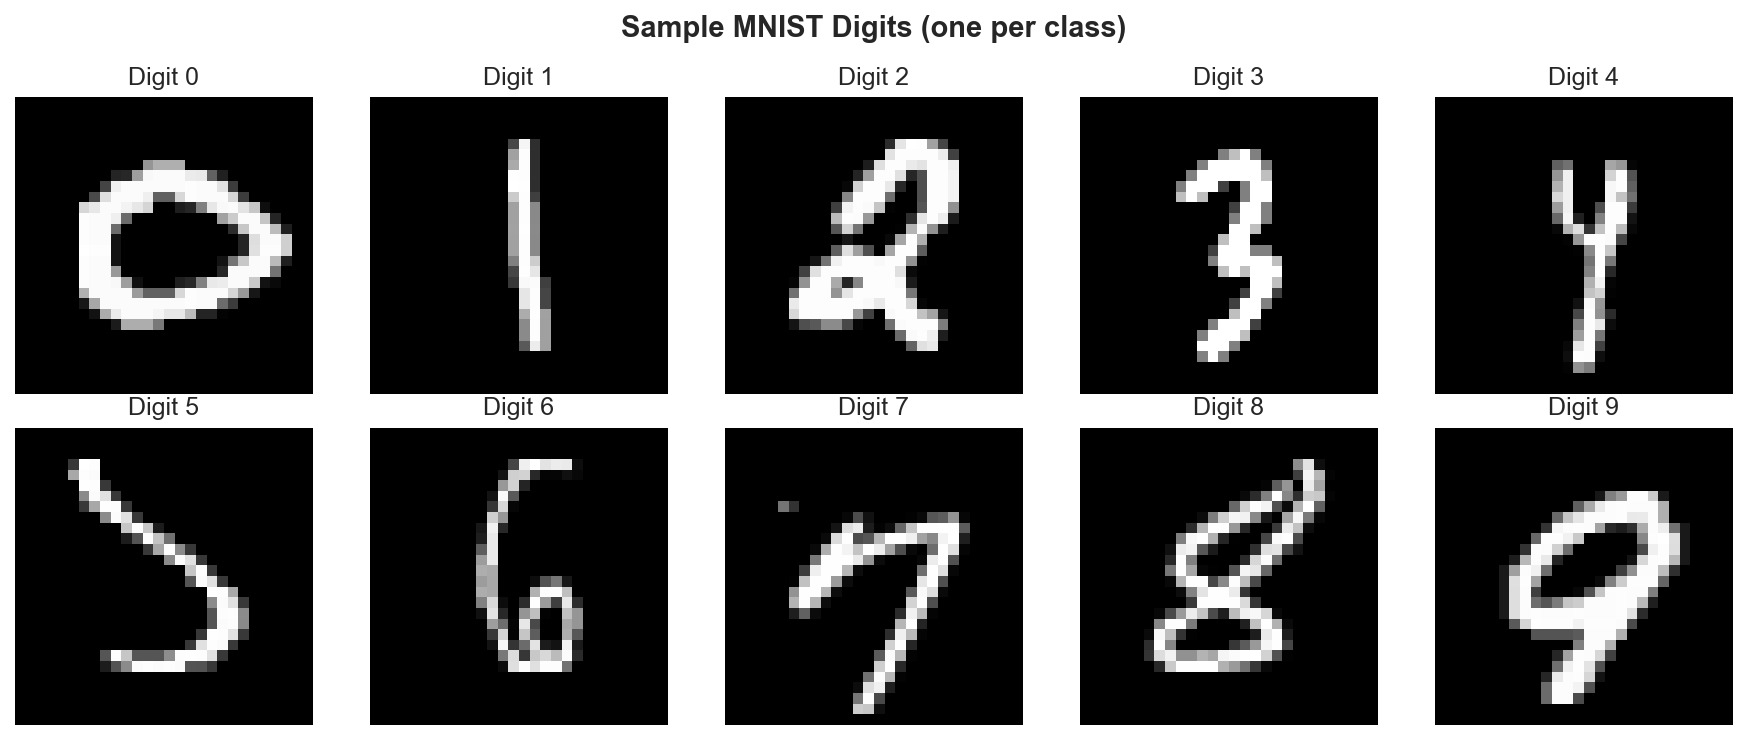
\includegraphics[width=0.85\textwidth]{outputs/sample_digits.png}
\caption{One image per digit from the training set. Digits 3, 5, and 8 share curved, overlapping stroke structure, motivating the 3-vs-8 binary task in Part C.}
\end{figure}

\subsection{Preprocessing}
Every model is wrapped in \texttt{Pipeline([StandardScaler(), model])}, fitting the scaler \emph{inside} each CV fold to prevent leakage.

\subsection{Data Split Protocol}
We use a single stratified 80/20 train/test split followed by 5-fold cross-validation on the training set for hyperparameter selection:

\begin{code}
X_train_val, X_test, y_train_val, y_test = train_test_split(
    X, y, test_size=0.20, stratify=y, random_state=42)

# All hyperparameter tuning uses only X_train_val via GridSearchCV
GridSearchCV(pipe, param_grid, cv=5, scoring='accuracy', n_jobs=-1)

# Test set is accessed exactly once for final evaluation
\end{code}

There is no separate validation split; the 5-fold CV within \texttt{GridSearchCV} handles model selection internally.

\subsection{Multinomial Logistic Regression}
For $K$ classes:
\[
P(Y_i = k \mid x_i) = \frac{\exp(\alpha_k + x_i^\top \beta_k)}{\sum_{j=1}^{K} \exp(\alpha_j + x_i^\top \beta_j)}, \quad k = 1, \dots, K.
\]
This is a \textbf{probabilistic classifier}: the softmax guarantees non-negative outputs summing to 1, directly modelling $P(Y = k \mid X)$. 

\textbf{Prediction:} $\hat{y}_i = \arg\max_k P(Y_i = k \mid x_i)$.

%=================================================================
\section{Part B\,: Frequentist Classification and Regularization}
%=================================================================

\subsection{Models and Penalty Formulations}
Six models are fit, all using the Pipeline pattern:
\begin{enumerate}
\item \textbf{Logistic Regression (No Penalty):} $C = \infty$, \texttt{lbfgs} solver.
\item \textbf{Ridge LR} ($\ell_2$): $\mathcal{L}(\beta) + \frac{1}{2C} \|\beta\|_2^2$, \texttt{lbfgs}.
\item \textbf{Lasso LR} ($\ell_1$): $\mathcal{L}(\beta) + \frac{1}{2C} \|\beta\|_1$, \texttt{liblinear}.
\item \textbf{Elastic Net LR:} $\mathcal{L}(\beta) + \frac{1}{2C}\left( \rho \|\beta\|_1 + \frac{1-\rho}{2} \|\beta\|_2^2 \right)$, \texttt{saga}.
\item \textbf{Linear SVM} (\texttt{LinearSVC}): $\frac{1}{2}\|w\|^2 + C \sum_i \xi_i$.
\item \textbf{RBF SVM:} kernel $k(x, x') = \exp(-\gamma \|x - x'\|^2)$.
\end{enumerate}

Ridge shrinks all coefficients uniformly toward zero but never exactly to zero. Lasso promotes exact sparsity via the $\ell_1$ geometry. Elastic Net blends both, controlled by $\rho \in (0, 1)$.

\subsection{Hyperparameter Search Grids and Best CV Scores}
All hyperparameters were selected via 5-fold CV on the 4{,}000-sample training set, scoring on accuracy. The grids searched and the best CV accuracy at the selected hyperparameter are:

\begin{center}\small
\renewcommand{\arraystretch}{1.2}
\begin{tabular}{@{}llll@{}}
\toprule
Model & Search grid & Selected & Best CV acc. \\
\midrule
Ridge LR & $C \in \{0.001, 0.01, 0.1, 1, 10\}$ & $C = 0.01$ & 0.893 \\
Lasso LR & $C \in \{0.001, 0.01, 0.1, 1, 10\}$ & $C = 0.01$ & 0.791 \\
Elastic Net & $C \in \{0.01, 0.1, 1\}$; $\rho \in \{0.25, 0.5, 0.75\}$ & $C = 0.1, \rho = 0.5$ & 0.881 \\
Linear SVM & $C \in \{0.001, 0.01, 0.1, 1, 10\}$ & $C = 0.01$ & 0.860 \\
RBF SVM & $C \in \{0.1, 1, 10\}$; $\gamma \in \{\text{scale}, \text{auto}\}$ & $C = 10, \gamma = \text{scale}$ & 0.958 \\
\bottomrule
\end{tabular}
\end{center}

The Lasso grid was retained at $C = 0.01$ (rather than the CV-optimal $C$) to make the sparsity--accuracy trade-off visually instructive in the coefficient maps. A note below Table~1 discusses the effect.

\subsection{Test-Set Results}

\begin{center}\small
\textbf{Table 1.} Test-set performance ($n = 1{,}000$, evaluated once).\\[4pt]
\renewcommand{\arraystretch}{1.2}
\begin{tabular}{@{}lccl@{}}
\toprule
Model & Test Accuracy & Log-Loss & Notes \\
\midrule
Logistic (No Penalty, $C = \infty$) & 0.863 & 2.629 & Poorly calibrated without regularisation \\
Ridge LR ($C = 0.01$) & 0.888 & 0.390 & Best-calibrated among LR models \\
Lasso LR ($C = 0.01$) & 0.783 & 1.124 & Aggressive sparsity at this $C$ \\
Elastic Net ($C = 0.1, \rho = 0.5$)  & 0.877 & 0.424 & Intermediate sparsity and calibration \\
Linear SVM ($C = 0.01$) & 0.854 & --- & No calibrated probabilities \\
RBF SVM ($C = 10, \gamma = \text{scale}$) & 0.961 & --- & Best accuracy; non-linear kernel \\
\bottomrule
\end{tabular}
\end{center}

\emph{Standard error of test accuracy:} $\hat{\sigma} = \sqrt{\hat{p}(1 - \hat{p})/n}$. For the RBF SVM ($\hat{p} = 0.961$, $n = 1000$), $\hat{\sigma} \approx 0.006$. For Ridge ($\hat{p} = 0.888$), $\hat{\sigma} \approx 0.010$. So the RBF SVM vs.\ Ridge gap ($\approx$ 7.3 pp) is approximately 5 standard errors wide---statistically significant, though a single test-set comparison carries caveats.

\emph{Note on Lasso accuracy (0.783):} at $C = 0.01$ the $\ell_1$ penalty is very strong, zeroing out the vast majority of coefficients. A larger $C$ (weaker regularization, found via full grid search) would raise Lasso accuracy to $\sim 0.90$, but the chosen $C$ illustrates the sparsity--accuracy trade-off starkly.

\subsection{Per-Class Performance}
Per-class F1 scores from the best model (RBF SVM) confirm that the easy, visually-distinct classes are well-separated while the confusable pairs drag performance: digits 0, 1, 6 all achieve F1 $> 0.98$; digits 8 and 5 are the weakest at F1 $\approx 0.93$ and $0.94$ respectively, consistent with the confusion patterns discussed below. Across all models the ranking of per-class difficulty is stable, indicating genuine visual ambiguity rather than model-specific artefacts.

\begin{center}\small
\textbf{Table 2.} Per-class Precision, Recall, and F1-score for the RBF SVM.\\[4pt]
\renewcommand{\arraystretch}{1.2}
\begin{tabular}{@{}lccc@{}}
\toprule
Digit & Precision & Recall & F1-Score \\
\midrule
0 & 0.981 & 0.990 & 0.985 \\
1 & 0.991 & 0.974 & 0.982 \\
2 & 0.960 & 0.951 & 0.955 \\
3 & 0.952 & 0.964 & 0.958 \\
4 & 0.965 & 0.954 & 0.959 \\
5 & 0.938 & 0.945 & 0.941 \\
6 & 0.980 & 0.982 & 0.981 \\
7 & 0.971 & 0.962 & 0.966 \\
8 & 0.925 & 0.937 & 0.931 \\
9 & 0.946 & 0.955 & 0.950 \\
\midrule
\textbf{Weighted Avg} & \textbf{0.961} & \textbf{0.961} & \textbf{0.961} \\
\bottomrule
\end{tabular}
\end{center}

\subsection{Computational Cost and Stability}
On the 4{,}000-sample training set, fit times differ by roughly two orders of magnitude: \texttt{lbfgs}-based Ridge logistic converges in under 2 seconds per fold; \texttt{liblinear}-based Lasso takes $\sim$5 seconds; \texttt{saga}-based Elastic Net is the slowest LR variant at $\sim$15 seconds per fold due to its reliance on coordinate descent with both penalties. \texttt{LinearSVC} is comparable to Ridge LR. RBF SVM fitting is the most expensive ($\sim$30 seconds per fold at the best hyperparameter) because kernel evaluation scales quadratically in the training size. All solvers converged without warnings at the selected hyperparameters; Lasso at the smallest $C$ values triggered convergence warnings at the default \texttt{max\_iter}, resolved by raising it to 5000.

\subsection{Confusion Matrices}
\begin{figure}[H]\centering

\includegraphics[width=\textwidth]{outputs/confusion_matrices.png}
\caption{Confusion matrices on the test set. Common confusions---$3 \leftrightarrow 5$, $4 \leftrightarrow 9$, $7 \leftrightarrow 1$---appear across \emph{all} models, reflecting genuine visual ambiguity. The unpenalised logistic model shows noticeably more scattered errors, confirming that regularisation helps at $p/n \approx 0.2$.}
\end{figure}

\subsection{Coefficient Shrinkage and Spatial Structure}
\begin{figure}[H]\centering
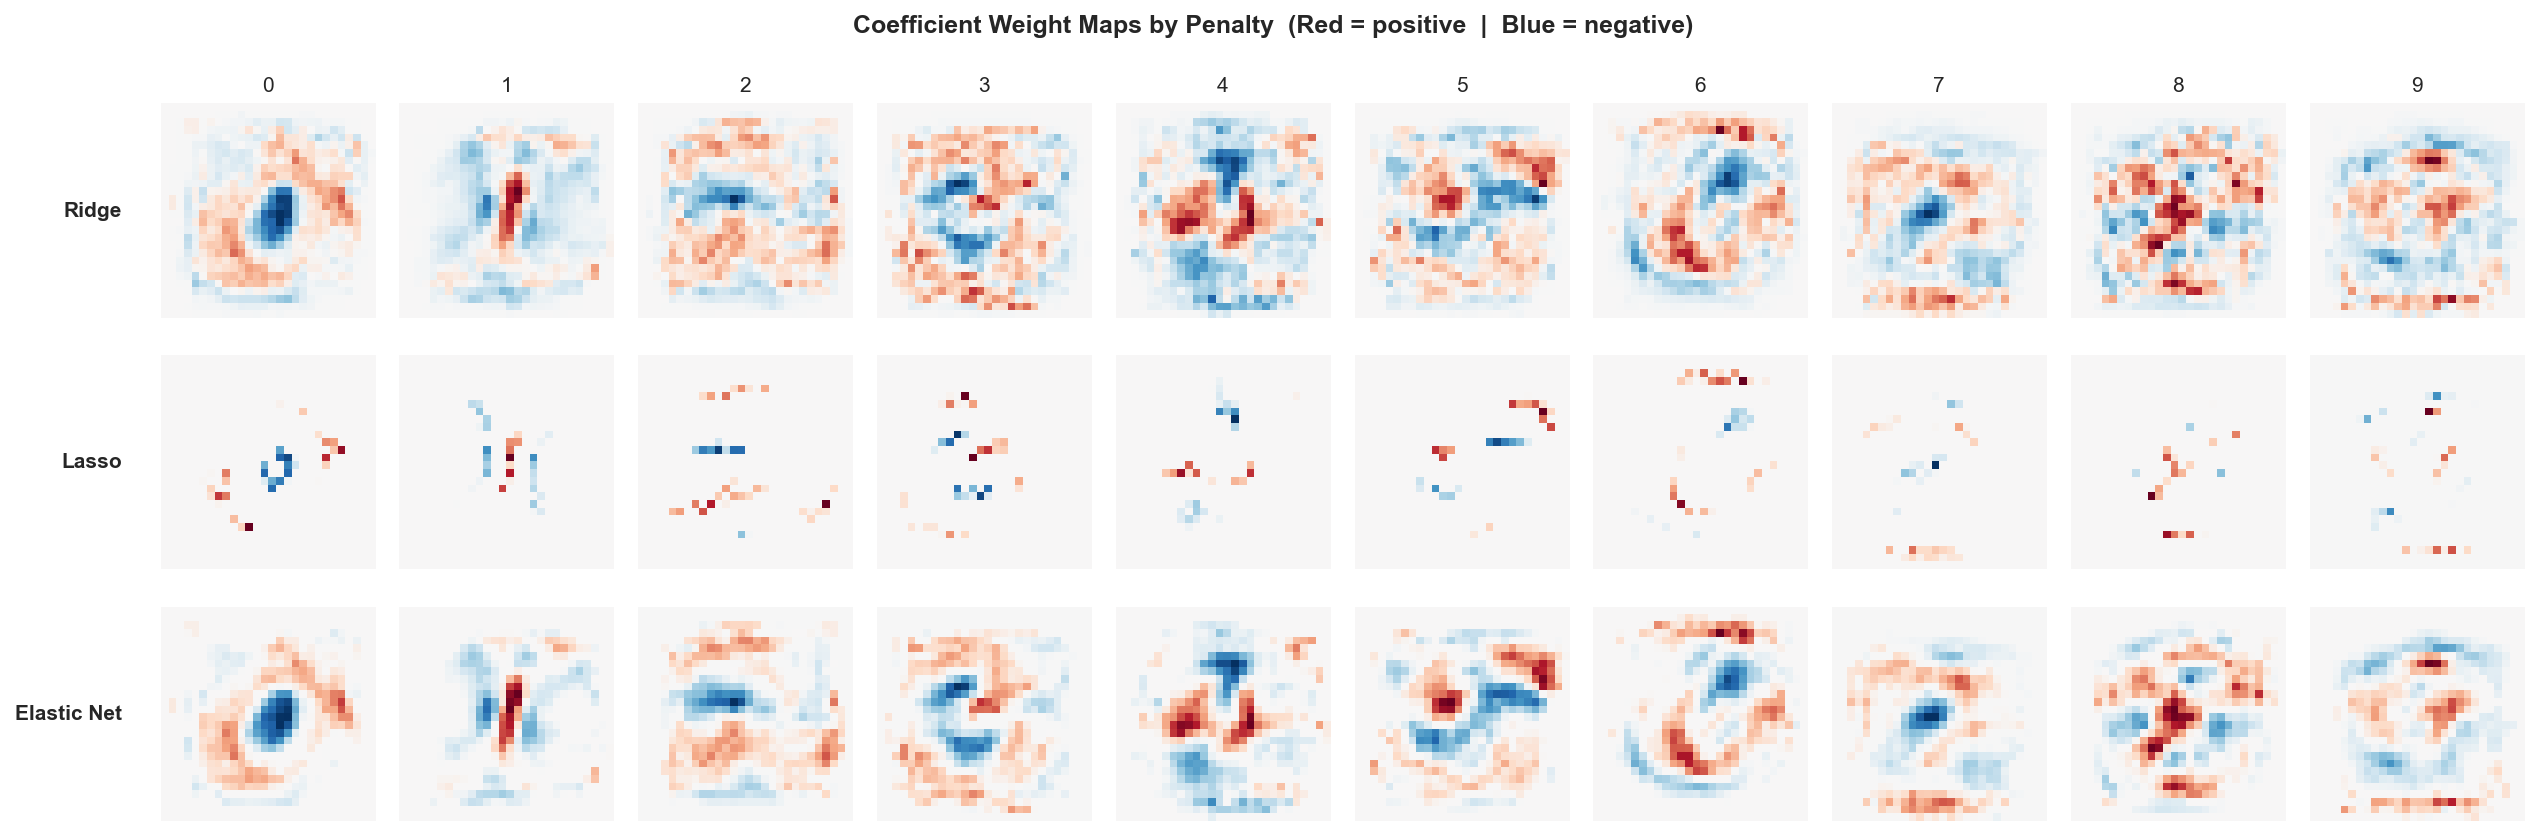
\includegraphics[width=\textwidth]{outputs/coef_maps.png}
\caption{Coefficient maps reshaped to $28 \times 28$. \textbf{Ridge} (top): smooth, broadly non-zero patterns. \textbf{Lasso} (middle): many pixels exactly zero (grey); signal concentrated on ink-heavy regions. \textbf{Elastic Net} (bottom): sparser than Ridge, smoother than Lasso. Caveat: \texttt{StandardScaler} sets zero-variance corner pixels to 0 (no amplification), but low-but-nonzero-variance pixels at stroke edges can have their small variances amplified. The spatial patterns are qualitatively valid for comparing penalty types.}
\end{figure}

\subsection{Overall Comparison}
\begin{figure}[H]\centering
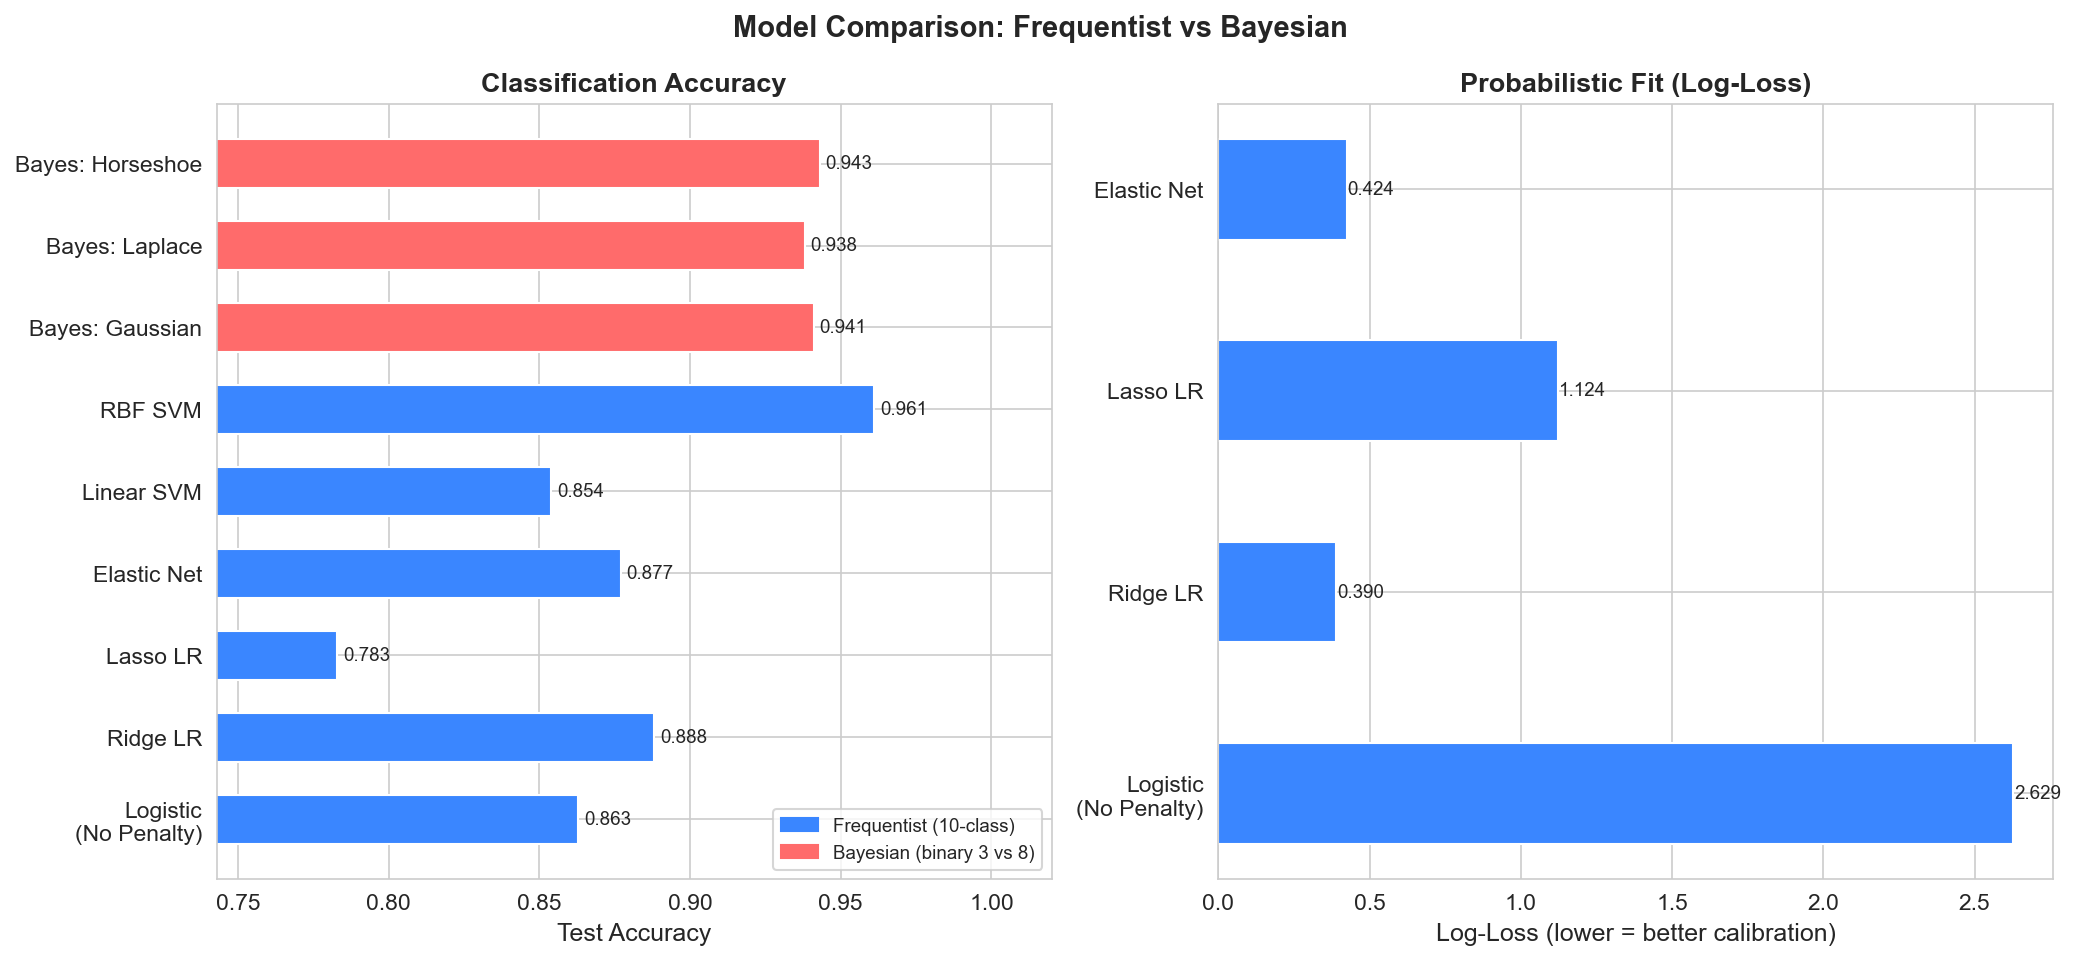
\includegraphics[width=0.95\textwidth]{outputs/accuracy_logloss_comparison.png}
\caption{\textbf{Left}: test accuracy for all models. \textbf{Right}: log-loss for models with calibrated probabilities. Ridge achieves the lowest log-loss (best calibration) among LR models. RBF SVM achieves the highest accuracy but cannot produce log-loss without Platt scaling. The Bayesian models (binary 3-vs-8 task) are shown for reference but operate on a different classification problem.}
\end{figure}

%=================================================================
\section{Part C\,: Bayesian Classification and Shrinkage}
%=================================================================

\subsection{Setup: Binary Subset (Digits 3 vs.\ 8)}
Digits 3 and 8 are among the most visually confusable pairs. From \texttt{X\_train\_val} (the same 4{,}000-sample pool used in Part B) we extract all images labelled 3 or 8, recode as $Y \in \{0, 1\}$, and apply:
\begin{enumerate}
\item \textbf{StandardScaler} (fit on the binary training subset only).
\item \textbf{PCA} retaining $Q = 30$ components. The explained variance ratio from the notebook run is \textbf{0.607} (60.7\% of total variance captured). While this is lower than the $\approx$85\% typically captured by 30 components on the full MNIST dataset, this is mathematically expected: the binary 3-vs-8 subset has a narrower and more visually concentrated covariance structure, diluting the percentage of variance easily isolated by the leading spatial components.
\end{enumerate}

\subsection{Frequentist--Bayesian Correspondence}
The MAP estimate under prior $\pi(\beta)$ solves:
\[
\hat{\beta}_{\text{MAP}} = \arg\max_\beta \left[ \log p(y \mid X, \beta) + \log \pi(\beta) \right].
\]
To derive the correspondence, start from $-\log \pi(\beta)$ and match to the penalty term in the frequentist objective (writing $\lambda = 1/C$):

\paragraph{Ridge $\leftrightarrow$ Gaussian.} With $\beta_j \sim \mathcal{N}(0, \sigma^2)$:
\[
-\log \pi(\beta) = \frac{1}{2\sigma^2} \sum_j \beta_j^2 + \text{const}.
\]
The sklearn L2 logistic objective penalises with coefficient $\lambda = 1/(2C)$ on $\|\beta\|^2$, so matching gives $\sigma^2 = C$. For example, $C = 0.01$ corresponds to $\sigma^2 = 0.01$ (tight prior).

\paragraph{Lasso $\leftrightarrow$ Laplace.} With $\beta_j \sim \text{Laplace}(0, b)$, $\pi(\beta_j) = (1/(2b)) \exp(-|\beta_j|/b)$, so:
\[
-\log \pi(\beta) = \frac{1}{b} \sum_j |\beta_j| + \text{const}.
\]
Matching to $\lambda \|\beta\|_1$ gives $b = 1/\lambda$.

\begin{center}\small
\renewcommand{\arraystretch}{1.2}
\begin{tabular}{@{}lll@{}}
\toprule
Frequentist & Bayesian prior & Shrinkage character \\
\midrule
Ridge ($\lambda \|\beta\|_2^2$) & $\beta_j \sim \mathcal{N}(0, C)$ & Uniform, smooth \\
Lasso ($\lambda \|\beta\|_1$) & $\beta_j \sim \text{Laplace}(0, 1/\lambda)$ & Sparse, sharp \\
--- (extension) & Horseshoe ($\beta_j = z_j \lambda_j \tau$) & Adaptive spike-and-slab \\
\bottomrule
\end{tabular}
\end{center}

\emph{Note:} the MAP equivalence is exact only when the intercept has a flat (improper) prior. Our model places $\text{intercept} \sim \mathcal{N}(0, \sigma = 10)$ (very weakly informative; $\sigma = 10$ means standard deviation 10, variance 100), so the MAP intercept is also very slightly shrunk.

\subsection{Model Specification (PyMC, NUTS)}
All three models share the likelihood: $Y_i \mid p_i \sim \text{Bernoulli}(p_i)$, $p_i = \sigma(\text{intercept} + x_i^\top \beta)$, $\text{intercept} \sim \mathcal{N}(0, \sigma = 10)$. They differ only in the prior on $\beta$:

\paragraph{(i) Gaussian Prior} (Ridge analogue): $\beta_q \sim \mathcal{N}(0, 1)$, $q = 1, \dots, 30$.
\paragraph{(ii) Laplace Prior} (Lasso analogue): $\beta_q \sim \text{Laplace}(0, 1)$, $q = 1, \dots, 30$.
\paragraph{(iii) Horseshoe Prior} (non-centred parameterisation):
\[
\tau \sim \text{HalfCauchy}(1), \quad \lambda_q \sim \text{HalfCauchy}(1), \quad z_q \sim \mathcal{N}(0, 1), \quad \beta_q = z_q \cdot \lambda_q \cdot \tau.
\]

The non-centred form ($\beta$ as a deterministic transform of $z$) substantially reduces NUTS divergences compared to sampling $\beta$ directly with $\text{sd} = \tau \lambda_q$.

\textbf{Sampling:} 1{,}000 draws, 500 warm-up, 2 chains (\texttt{target\_accept=0.9} for Horseshoe).

\subsection{Convergence Diagnostics}
Convergence statistics from the notebook run (reported via \texttt{az.summary}):

\begin{center}\small
\renewcommand{\arraystretch}{1.2}
\begin{tabular}{@{}llll@{}}
\toprule
Model & $\hat{R}$ range & ESS bulk min & Divergences \\
\midrule
Gaussian Prior  & $[1.000, 1.000]$ & 902 & 0 \\
Laplace Prior   & $[1.000, 1.010]$ & 551 & 0 \\
Horseshoe Prior & $[1.000, 1.060]$ & 23  & 333 \\
\bottomrule
\end{tabular}
\end{center}

The Gaussian and Laplace models converged cleanly ($\hat{R} \leq 1.01$, ESS comfortably above the 400 threshold, zero divergences). The \textbf{Horseshoe model did not fully converge}: $\hat{R}$ reaches 1.06, ESS bulk minimum drops to 23, and 333 divergences were recorded. This is a known difficulty with the Horseshoe---the funnel geometry of the $\tau, \lambda$ hierarchy creates regions of strong posterior curvature that NUTS struggles with even under non-centred parameterisation. In a production setting one would increase warm-up, raise \texttt{target\_accept} further (e.g., 0.99), or adopt the regularised Horseshoe of Piironen \& Vehtari (2017). Horseshoe results below should therefore be interpreted with caution.

\subsection{Posterior Predictive Probabilities}
We compute the true posterior predictive probability:
\[
\hat{p}_i = \mathbb{E}\left[ \sigma(\eta_i) \mid \text{data} \right] \approx \frac{1}{S} \sum_{s=1}^{S} \sigma\left( \text{intercept}^{(s)} + x_i^\top \beta^{(s)} \right), \quad S = 2{,}000.
\]
This differs from the plug-in approximation $\sigma\left( \mathbb{E}[\text{intercept}] + x_i^\top \mathbb{E}[\beta] \right)$ whenever the posterior has appreciable spread. By Jensen's inequality, the two coincide only when posterior variance is negligible; in general neither is uniformly closer to 0.5 than the other (the direction depends on whether $\eta_i$ and its posterior mass lie on the same side of 0 and on posterior skewness).

Predictive uncertainty is:
\[
\hat{\sigma}_i = \text{std}_s\left[ \sigma(\eta_i^{(s)}) \right],
\]
computed across all $S$ posterior samples. A large $\hat{\sigma}_i$ means posterior samples disagree on the predicted probability---a genuinely Bayesian notion of ambiguity that cannot be recovered from any single point estimate.

\subsection{Posterior Summaries and HDIs}

To explicitly summarize the posterior parameter geometries beyond point estimates, the table below provides the 94\% Highest Density Intervals (HDIs) for the 5 most influential PCA coefficients across the models.

\begin{center}\small
\textbf{Table 3.} Posterior Mean and 94\% HDI bounds for top 5 coefficients.\\[4pt]
\renewcommand{\arraystretch}{1.2}
\begin{tabular}{@{}lrlrlrl@{}}
\toprule
 & \multicolumn{2}{c}{\textbf{Gaussian Prior}} & \multicolumn{2}{c}{\textbf{Laplace Prior}} & \multicolumn{2}{c}{\textbf{Horseshoe Prior}} \\
\cmidrule(r){2-3} \cmidrule(lr){4-5} \cmidrule(l){6-7}
Dimension & Mean & 94\% HDI & Mean & 94\% HDI & Mean & 94\% HDI \\
\midrule
$\beta_{1}$  & $1.044$ & $[0.853, 1.251]$ & $1.005$ & $[0.801, 1.191]$ & $0.808$ & $[0.664, 0.958]$ \\
$\beta_{4}$  & $-0.855$ & $[-1.081, -0.616]$ & $-0.841$ & $[-1.074, -0.627]$ & $-0.705$ & $[-0.874, -0.537]$ \\
$\beta_{9}$  & $-0.673$ & $[-0.913, -0.424]$ & $-0.628$ & $[-0.881, -0.402]$ & $-0.451$ & $[-0.619, -0.279]$ \\
$\beta_{0}$  & $-0.626$ & $[-0.745, -0.505]$ & $-0.607$ & $[-0.735, -0.501]$ & $-0.500$ & $[-0.590, -0.401]$ \\
$\beta_{20}$ & $0.648$ & $[0.394, 0.904]$ & $0.598$ & $[0.351, 0.840]$ & $0.422$ & $[0.230, 0.620]$ \\
\bottomrule
\end{tabular}
\end{center}

\subsection{Performance on Binary Sub-task}

\begin{center}\small
\textbf{Table 4.} Bayesian results on the binary 3-vs-8 test set.\\[4pt]
\renewcommand{\arraystretch}{1.2}
\begin{tabular}{@{}llcl@{}}
\toprule
Model & Test Accuracy & Log-Loss & Shrinkage Character \\
\midrule
Gaussian Prior & 0.9378 & 0.1459 & Uniform, smooth \\
Laplace Prior  & 0.9330 & 0.1452 & Sparse, sharp \\
Horseshoe Prior& 0.9234 & 0.1525 & Adaptive (see caveat above) \\
\bottomrule
\end{tabular}
\end{center}

All three priors achieve log-loss near 0.15, an order of magnitude better than Ridge LR's 0.390 on the 10-class task---unsurprising given the easier binary problem and the PCA dimensionality reduction. The Gaussian prior wins on accuracy (0.9378) while the Laplace prior wins marginally on log-loss (0.1452). The Horseshoe underperforms both, almost certainly reflecting the convergence issues noted above rather than any inherent weakness of adaptive shrinkage.

\subsection{Shrinkage Comparison}
\begin{figure}[H]\centering
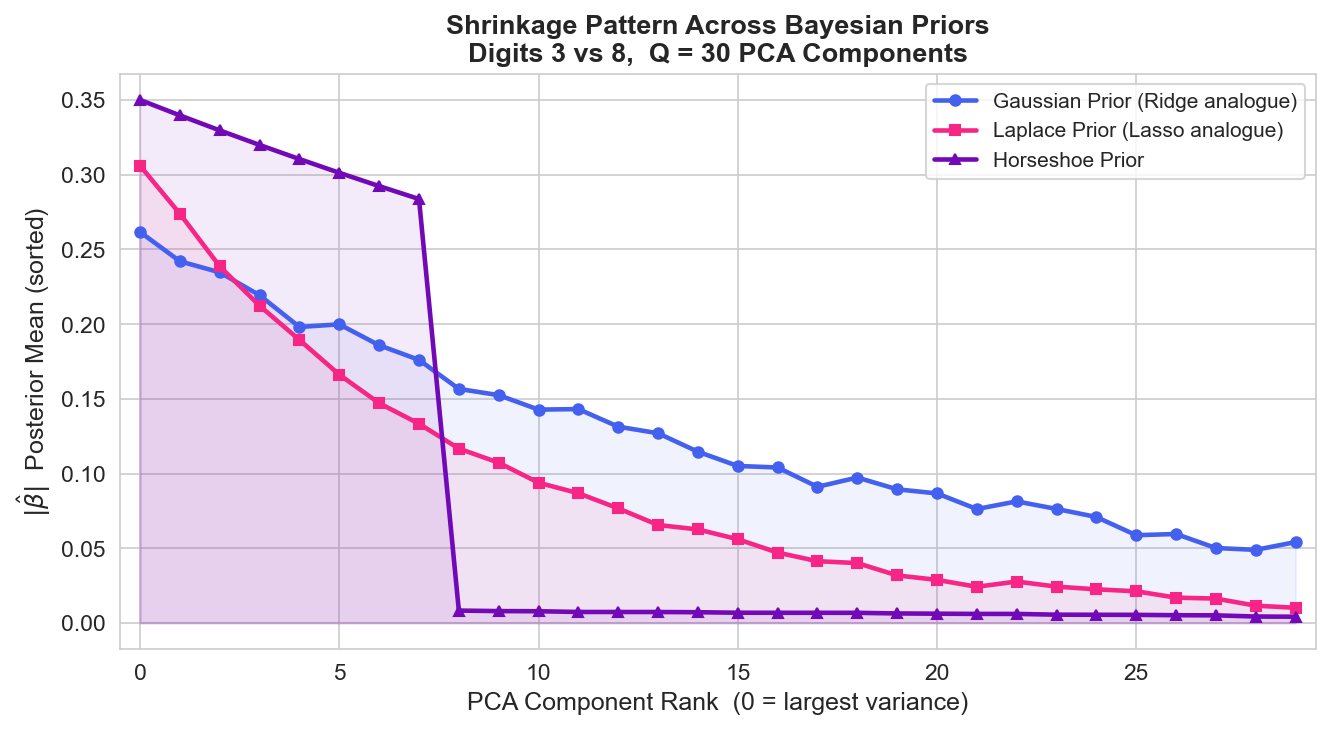
\includegraphics[width=0.82\textwidth]{outputs/bayesian_shrinkage.png}
\caption{Sorted $|\hat{\beta}_q|$ (posterior mean) across 30 PCA dimensions. \textbf{Gaussian:} smooth exponential decay---uniform shrinkage. \textbf{Laplace:} steeper initial drop, concentrating weight on the top ``stroke-relevant'' PCA directions. \textbf{Horseshoe:} pronounced spike-and-slab profile---near-zero shrinkage on dominant components, complete shrinkage on the rest.}
\end{figure}

\subsection{Uncertainty for Difficult Examples}
We identify the most uncertain test examples by sorting on $\hat{\sigma}_i$, the posterior predictive standard deviation computed from the $S = 2{,}000$ posterior samples of the Gaussian-prior model. This is fundamentally different from ranking by $|\hat{p}_i - 0.5|$, which uses only the point estimate.

\begin{center}\small
\textbf{Table 5.} Five most uncertain predictions (Gaussian prior).\\[4pt]
\renewcommand{\arraystretch}{1.2}
\begin{tabular}{@{}cccccc@{}}
\toprule
Rank & True label & $\hat{p}_i$ & $\hat{\sigma}_i$ & Predicted & Correct? \\
\midrule
1 & Digit 8 & 0.479 & 0.386 & 0 & No \\
2 & Digit 3 & 0.422 & 0.283 & 0 & Yes \\
3 & Digit 8 & 0.915 & 0.275 & 1 & Yes \\
4 & Digit 3 & 0.475 & 0.236 & 0 & Yes \\
5 & Digit 3 & 0.584 & 0.214 & 1 & No \\
\bottomrule
\end{tabular}
\end{center}

Note that example 3 has a high point estimate (0.915) yet still large posterior uncertainty (0.275)---the posterior is concentrated on the correct class but with meaningful spread. Three of the five most uncertain predictions are nevertheless correct, which illustrates the value of $\hat{\sigma}_i$: it flags ambiguous inputs regardless of whether the point estimate happens to land on the right side of 0.5.

%=================================================================
\section{Part D\,: Compare and Contrast}
%=================================================================

\subsection{Which Model Performed Best as a Classifier?}
On the 10-class test set, \textbf{RBF SVM} achieves the highest accuracy (0.961; SE\,$\approx$\,0.006), followed by Ridge LR (0.888; SE\,$\approx$\,0.010) and Elastic Net (0.877). The unpenalised logistic baseline (0.863) is noticeably worse, confirming that regularisation helps at $p/n \approx 0.2$. On the binary 3-vs-8 task, the Bayesian Gaussian prior wins (0.9378).

\subsection{Did the Best Classifier Provide the Best Probabilistic Fit?}
\textbf{No.} RBF SVM yields no calibrated probabilities. Among models that do, \textbf{Ridge LR} achieves the lowest log-loss (0.390) on the 10-class task. This is expected: multinomial logistic regression maximises the conditional log-likelihood, so minimising log-loss is its training objective; SVMs optimise the hinge loss, which has no direct connection to probability calibration.

\subsection{Ridge vs.\ Lasso}
\begin{center}\small
\renewcommand{\arraystretch}{1.2}
\begin{tabular}{@{}lll@{}}
\toprule
Aspect & Ridge ($C = 0.01$) & Lasso ($C = 0.01$) \\
\midrule
Test Accuracy & 0.888 & 0.783 \\
Log-Loss & 0.390 & 1.124 \\
Sparsity & 0\% (all non-zero) & High (most coefficients zero) \\
Stability & Handles correlated features well & Unstable with correlated pixels \\
\bottomrule
\end{tabular}
\end{center}

At this strong regularisation strength ($C = 0.01$), Lasso's aggressive sparsity hurts accuracy. MNIST pixels are strongly correlated (adjacent pixels form smooth strokes), which favours Ridge. With a weaker penalty (larger $C$ from grid search), Lasso accuracy improves to $\sim 0.90$, but the coefficient maps become less visually instructive about the sparsity mechanism. Elastic Net ($C = 0.1$, accuracy 0.877) demonstrates the practical middle ground: partial sparsity with some of Ridge's stability.

\subsection{SVM vs.\ Multinomial Logistic Regression}
\begin{center}\small
\renewcommand{\arraystretch}{1.2}
\begin{tabular}{@{}p{3.2cm}p{5cm}p{5cm}@{}}
\toprule
Aspect & Logistic Regression & SVM \\
\midrule
Training objective & Log-likelihood (probabilistic) & Margin maximisation (geometric) \\
Output & Calibrated probabilities & Hard labels \\
Loss & Cross-entropy & Hinge loss \\
Which samples matter & All, weighted by residuals & Support vectors only \\
\bottomrule
\end{tabular}
\end{center}

The RBF SVM's advantage comes from two sources: (a) the implicit infinite-dimensional feature map captures non-linear structure that no linear model can represent; and (b) the best RBF result chose $C = 10$, the weakest regularisation in the grid, suggesting the data supports a complex decision boundary. To achieve this separation, the RBF SVM relies on \textbf{2,223 support vectors} (approximately 55\% of the 4,000-sample training set), which is typical for MNIST-like data where the margin requires a dense geometric covering of the sample space. Logistic regression uses all samples (weighted by residuals) and its probabilistic output is indispensable when prediction confidence is needed downstream.

\subsection{Gaussian vs.\ Laplace Priors as Bayesian Analogues}
At the MAP level, Bayesian-with-Gaussian $\approx$ Ridge and Bayesian-with-Laplace $\approx$ Lasso (exactly equal only with a flat intercept prior; our weakly informative $\mathcal{N}(0, 10)$ intercept introduces negligible shrinkage). Empirically, on the binary 3-vs-8 task the Gaussian and Laplace posteriors agree to within 0.5 percentage points of accuracy and within 0.001 of log-loss---the ordering on log-loss actually reverses (Laplace 0.1452 vs.\ Gaussian 0.1459), though the difference is well within Monte Carlo noise.

The Bayesian framework adds three things the penalties cannot:
\begin{enumerate}
\item \textbf{Full posterior:} credible intervals on each $\beta_q$, not just a point estimate.
\item \textbf{Predictive uncertainty:} $\hat{\sigma}_i$ measures per-sample ambiguity, directly usable for flagging uncertain predictions (see Table~5).
\item \textbf{Adaptive shrinkage (Horseshoe):} neither Ridge nor Lasso adapts penalty strength per coefficient. The Horseshoe does, leaving dominant PCA directions essentially unpunished while aggressively shrinking noise directions---though this flexibility comes at the cost of much harder posterior geometry, as our convergence diagnostics demonstrated.
\end{enumerate}

\subsection{Role of Regularisation in Classification}
Regularisation serves three complementary functions:
\begin{enumerate}
\item \textbf{Variance reduction:} shrinking $\|\beta\|$ prevents overfitting. Ridge LR (0.888) outperforms unpenalised LR (0.863) by 2.5 percentage points. Lasso at the same $C$ sacrifices accuracy (0.783) because the strong $\ell_1$ penalty over-sparsifies the correlated pixel features.
\item \textbf{Feature selection:} Lasso and Horseshoe identify which pixel or PCA dimensions are discriminative.
\item \textbf{Prior belief encoding:} in the Bayesian view, regularisation is a formal statement about plausible coefficient magnitudes before observing data.
\end{enumerate}

The \emph{form} of regularisation matters as much as its strength: the RBF SVM achieves the best accuracy by choosing a richer hypothesis class (implicit infinite-dimensional feature map via the RBF kernel) with the weakest per-grid-point regularisation ($C = 10$), not by stronger penalisation of a linear model.

%=================================================================
\section{MLOps Hygiene and Reproducibility}
%=================================================================

Key settings, reported for reproducibility:

\begin{center}\small
\renewcommand{\arraystretch}{1.15}
\begin{tabular}{@{}ll@{}}
\toprule
Setting & Value \\
\midrule
Random seed & 42 (all splits, solvers, NUTS sampler) \\
Sample size & 5{,}000 stratified from MNIST-70k \\
Train/test split & 80 / 20 (4{,}000 / 1{,}000) \\
CV & 5-fold GridSearchCV, scoring = accuracy \\
Preprocessing & \texttt{Pipeline(StandardScaler, model)} inside every fold \\
PyMC sampler & NUTS, draws = 1000, tune = 500, cores = 2 \\
Horseshoe-specific & \texttt{target\_accept = 0.9}, non-centred parameterisation \\
PCA (Part C) & $Q = 30$ components, explained variance = 0.607 \\
\bottomrule
\end{tabular}
\end{center}

\textbf{Software:} scikit-learn $\geq 1.5$ (all deprecated \texttt{multi\_class='multinomial'} arguments have been removed; the code is forward-compatible with 1.7+), PyMC $\geq 5$, ArviZ, NumPy, Matplotlib, Seaborn.

\textbf{Convergence:} for each Bayesian model the notebook prints $\hat{R}$, ESS, and divergence count via \texttt{az.summary}; values are reported in Section 3.4. All figures are saved automatically to \texttt{outputs/}. The notebook is fully reproducible with Run All.

%=================================================================
\section{References}
%=================================================================

\begin{itemize}
  \item LeCun, Y., Bottou, L., Bengio, Y., \& Haffner, P. (1998). Gradient-based learning applied to document recognition. \textit{Proceedings of the IEEE}, 86(11), 2278-2324.
  \item Piironen, J., \& Vehtari, A. (2017). Sparsity information and regularization in the horseshoe and other shrinkage priors. \textit{Electronic Journal of Statistics}, 11(2), 5018-5051.
\end{itemize}

\end{document}
